\textbf{Ejemplo 7}\\
Suponga que una cuenta de ahorros de un banco le paga una tasa nominal anual año vencido del 24\%.
¿Cuál sería la tasa periódica día vencido? Asuma un año de 365 días.\\

%\newpage %USAR SOLO SI EL SOLUCIÓN QUEDA SOLO Y ES NECESARIO BAJARLO A LA SIGUIENTE PAGINA
\textbf{Solución.}\\
%La tabla ira centrada
\begin{center}
  \renewcommand{\arraystretch}{1.5}% Margenes de las celdas
  %Creación de la cuadricula de 3 columnas
  \begin{longtable}[H]{|C{0.3\linewidth}|C{0.3\linewidth}|C{0.3\linewidth}|}
    %Creamos una linea horizontal
    \hline

    %%%%% INICIO ASIGNACIÓN PERíODO FOCAL %%%%%%%
    %%%%%%%%%% INICIO TITULO
    \rowcolor[HTML]{FFB183}
    \multicolumn{3}{|c|}{\cellcolor[HTML]{FFB183}\textbf{1. Asignación período focal}}                                                                                             \\ \hline
    \multicolumn{3}{|c|}{$pf: \textit{No aplica}$}                                                                                                                                 \\ \hline

    %%%%%%%%%% FIN TITULO
    %%%%% INICIO DECLARACIÓN DE VARIABLES %%%%%%%
    %%%%%%%%%% INICIO TITULO
    %Lo que se hace aquí es mezclar las 3 columnas en una sola
    \multicolumn{3}{|c|}{\cellcolor[HTML]{FFB183}\textbf{2. Declaración de variables}}                                                                                             \\ \hline
    %%%%%%%%%% FIN TITULO
    %%%%%%%%%% INICIO SUBTITULO
    \cellcolor[HTML]{FFB183}\textbf{Valores monetarios}    & 
    \cellcolor[HTML]{FFB183}\textbf{Valores no monetarios} &
    \cellcolor[HTML]{FFB183}\textbf{Incógnitas}  \\ \hline
    %%%%%%%%%% FIN SUBTITULO
    %%%%%%%%%% INICIO DE MATEMÁTICAS
    %Cada & hace referencia al paso de la siguiente columna
    $j_{1}= 24\% \textit{ naav}$ & $m_{1} = 1 \textit{ ptv}$ & $i_{2} = ?\% \textit{ pdv} $ \\
    $i_{1}= 24\% \textit{ ptv}$ &  $m_{2} = 365 \textit{ pdv} $ & \\ 
         &      & \\ \hline

    %%%%%%%%%% FIN DE MATEMÁTICAS
    %%%%% FIN DECLARACIÓN DE VARIABLES


    %%%%% INICIO FLUJO DE CAJA
    \rowcolor[HTML]{FFB183}
    \multicolumn{3}{|c|}{\cellcolor[HTML]{FFB183}\textbf{3. Diagrama de equivalencia de tasas}}                                                                                    \\ \hline
    %Mezclamos 3 columnas y pondremos el dibujo
    %%%%%%%%%%%%% INSERCIÓN DE LA IMAGEN
    %Deberán descargar las imágenes respectivas del drive y pegarlas en la carpeta
    %n_capitulo/img/ejemplos/1/capitulo1ejemplo1.pdf  (el /1/ es el numero del ejemplo)

    \multicolumn{3}{|c|}{ 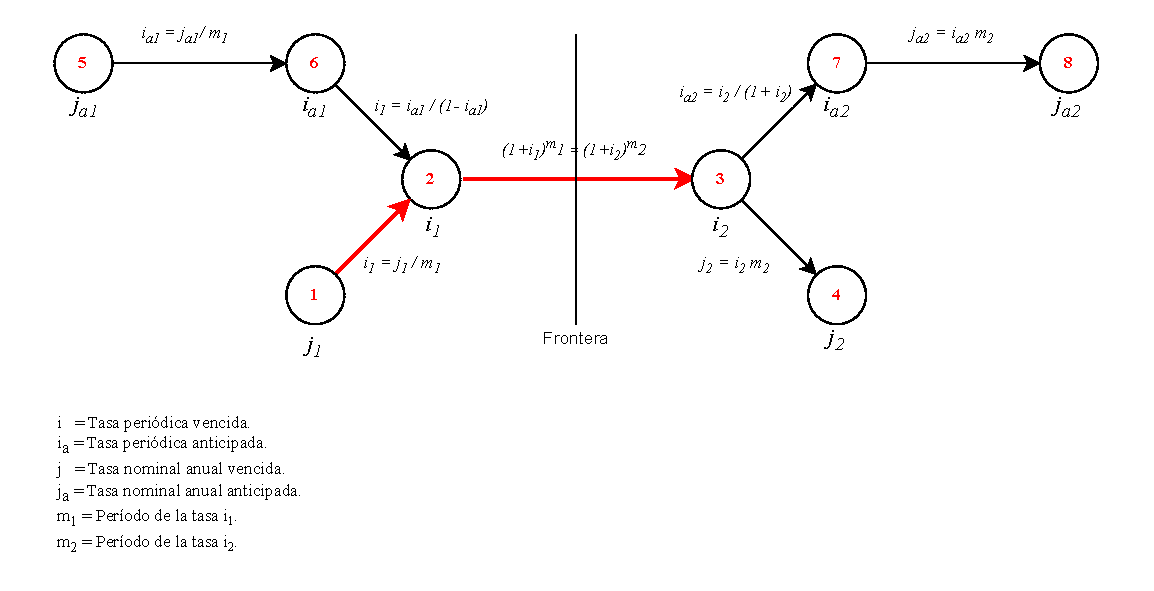
\includegraphics[height = 7.0 cm]{2_Capitulo/ejemplos/7/Capitulo2Ejercicio7.pdf} } \\ \hline
    
    %%%%%%%%%%%%% FIN INSERCIÓN DE IMAGEN
    %%%%%FIN FLUJO DE CAJA

    %%%%% INICIO DECLARACIÓN FORMULAS
    %%%%%%%%%%% INICIO TITULO
    \rowcolor[HTML]{FFB183}
    \multicolumn{3}{|c|}{\cellcolor[HTML]{FFB183}\textbf{4. Declaración de fórmulas}}                                                                                              \\ \hline
    %%%%%%%%%%% FIN TITULO
    %%%%%%%%%%% INICIO MATEMÁTICAS

    \multicolumn{3}{|c|}{$(1+i_{1})^{m_{1}} = (1+i_{2})^{m_{2}} \hspace{0.3cm} \textit{ Equivalencia de tasas}$}                                \\ \hline
    %%%%%%%%%% FIN MATEMÁTICAS
    %%%%%% INICIO DESARROLLO MATEMÁTICO
    \rowcolor[HTML]{FFB183}
    %%%%%%%%%%INICIO TITULO
    \multicolumn{3}{|c|}{\cellcolor[HTML]{FFB183}\textbf{5. Desarrollo matemático}}                                                                                                \\ \hline
    %%%%%%%%%% FIN TITULO
    %%%%%%%%%% INICIO MATEMÁTICAS
    \multicolumn{3}{|c|}{$(1 + 0,24)^{1}= (1 + i_{2})^{365}$}                                            \\
    \multicolumn{3}{|c|}{$(1,24)^\frac{1}{365}-1 = i_{2}$} \\ 
    \multicolumn{3}{|c|}{$i_{2}=1.00059-1 \textit{ pdv}$} \\
    \multicolumn{3}{|c|}{$i_{2}=0.00059 \textit{ pdv} \equiv 0.059\% \textit{ pdv}$} \\

    %%%%%%%%%% FIN MATEMÁTICAS
    %%%%%% FIN DESARROLLO MATEMÁTICO
    %%%%%% INICIO RESPUESTA
    \rowcolor[HTML]{FFB183}
    %%%%%%%%%%INICIO TITULO
    \multicolumn{3}{|c|}{\cellcolor[HTML]{FFB183}\textbf{6. Respuesta}}                                                                                                            \\ \hline
    %%%%%%%%%% FIN TITULO
    %%%%%%%%%% INICIO RESPUESTA MATEMÁTICA
    \multicolumn{3}{|c|}{${i_{2} = 0,059\% \textit{ pdv}}$}\\ \hline
    %%%%%%%%%% FIN MATEMÁTICAS
    %%%%%% FIN RESPUESTA
  \end{longtable}
  %Se crean dos lineas en blanco para que no quede el siguiente texto tan pegado
  %\newline \newline %USARLO SI CREES QUE ES NECESARIO
\end{center}
%%%%%%%%%%%%%%%%%%%%%%%%%%FIN EJERCICIO 7 %%%%%%%%%%%%%%%%%%%%%%%%%%%